% This is LLNCS.DOC the documentation file of
% the LaTeX2e class from Springer-Verlag
% for Lecture Notes in Computer Science, version 2.4
\documentclass{llncs}

\usepackage{llncsdoc}
\let \proof \relax
\let\endproof\relax
\usepackage{amsthm,amsmath}
\usepackage{graphicx}
\usepackage{multirow}
\usepackage{booktabs}
\usepackage{subfig}
%\usepackage{subfigure}
\usepackage{lipsum}
\usepackage{array}
\usepackage{algorithm}
\usepackage{algorithmic}
\usepackage{color,soul}
\usepackage{epstopdf}
%\newcolumntype{L}[1]{>{\raggedright\let\newline\\\arraybackslash\hspace{0pt}}m{#1}}
%\newcolumntype{C}[1]{>{\centering\let\newline\\\arraybackslash\hspace{0pt}}m{#1}}
%\newcolumntype{R}[1]{>{\raggedleft\let\newline\\\arraybackslash\hspace{0pt}}m{#1}}
\renewcommand{\algorithmicrequire}{\textbf{Input:}}
\renewcommand{\algorithmicensure}{\textbf{Output:}}
%\newcommand{\algorithmicbreak}{\textbf{break}}
%\newtheorem{theorem}{Theorem}
%\newtheorem{corollary}{Corollary}
%\newtheorem{lemma}{Lemma}
%
\begin{document}

\title{Fast Generalized Distillation for Semi-supervised Domain Adaptation}
\maketitle
\begin{abstract}
	Semi-supervised domain adaptation (SDA) is a typical setting when we face the problem of domain adaptation in real applications. How to effectively utilize the unlabeled data is an important issue in SDA. In this paper, we propose a new paradigm, called \textit{Generalized Distillation Semi-supervised Domain Adaptation} (GDSDA) to solve the SDA problem.
	We first demonstrate that GDSDA can effectively utilize the unlabeled data to transfer the knowledge from the source models. We illustrate that the imitation parameter of GDSDA can greatly affect the performance of the target model and propose GDSDA-SVM which uses SVMs as the base classifier and can effectively estimate the imitation parameter. Specifically, the imitation parameter is estimated by minimizing the Leave-one-out cross-validation loss on the target data using our novel objective function. Experiment results show that GDSDA-SVM can effectively utilize the unlabeled data to transfer the knowledge between different domains under the SDA setting.
\end{abstract}

\section{Introduction}
Domain adaptation can be used in many real applications, which addresses the problem of learning a target domain with the help of a different but related source domain. 
In real applications, it can be very expensive to obtain sufficient labeled examples while there are abundant unlabeled ones. 
\textit{Semi-supervised domain adaptation} (SDA) tries to exploit the knowledge from the source domain and use a certain amount of unlabeled examples and a few labeled ones from the target domain to learn a target model. Typically, the labeled examples in the target domain are too few to construct a good classifier alone. Therefore, an important issue in SDA is how to effectively utilize the unlabeled examples.

In previous work, many methods have been proposed to leverage the source knowledge with the unlabeled data.
Duan et al.\cite{duan2009domain} proposed a method to force the source models and the target model to agree on the unlabeled data. Daum{\'e} et al\cite{daume2010frustratingly} utilized unlabeled data as a co-regularizer and forced the hypotheses learned from different domains to agree on the unlabeled data. Meanwhile, Yao et al.\cite{yao2015semi} used the unlabeled target examples to discover the underlying intrinsic information in the target domain. Donahue et al.\cite{Donahue_2013_CVPR} show that using the smoothness constraints on the classifier scores over the unlabeled data can lead to the improved transfer result.
The previous work in SDA requires access to the source data to measure the data distribution mismatch between the source and target domain.
However, in some situations, we may not be able to access each of the source examples for many reasons. When we use a large dataset as our source domain, for example, it is ineffective to compare each of the source examples with the target data to estimate the data distribution mismatch.

Recently, a framework called \textit{Generalized Distillation} (\textbf{GD})\cite{lopez2015unifying} was proposed, which allows the knowledge to be transferred between different models effectively. GD includes two different models, the teacher model and student model. The student model tries to learn from the teacher model by mimicking the outputs of the teacher model on the training data. Remarkably, in GD, the knowledge can be directly transferred from the teacher model to the student model without accessing the data used to train the teacher. Moreover, GD can be used to exploit the information of the unlabeled data in a semi-supervised scenario\cite{lopez2015unifying}.
Given that GD has such ability, it is natural to ask the following two questions: (1) Can the GD framework be applied to solve the SDA problem? (2) How can we improve its effectiveness when we apply GD to real SDA applications?

To answer these two questions, in this paper, we first propose a new paradigm, called \textit{Generalized Distillation Semi-supervised Domain Adaptation} (\textbf{GDSDA}), to solve the SDA problem. 
We show that, with GDSDA the knowledge of the source models can be effectively transferred to the target domain using the unlabeled data. Specifically, the target model is trained with the help of the soft labels, i.e. the predictions of the target domain examples given by the source models. Therefore, without accessing each of the source examples, GDSDA is more efficient especially when the source domain is relatively large and the source model is well-trained.

Then we argue that the imitation parameter of GDSDA which controls the amount of knowledge transferred from the source model can greatly affect the performance of the target model.
However, according to the previous work\mbox{\cite{lopez2015unifying,Tzeng_2015_ICCV}}, the imitation parameter is a hyperparameter and can only be determined by either brute force search or background knowledge. 
Therefore, we propose a novel imitation parameter estimation method for GDSDA, called GDSDA-SVM, which uses SVM as the base classifier and determines the imitation parameter efficiently. In particular, we use the Mean Square Error loss for GDSDA-SVM and show that the Leave-one-out cross validation (LOOCV) loss can be calculated in a closed form. By minimizing the LOOCV loss on the target data, we can find the optimal imitation parameter. In our experiments, we show that GDSDA-SVM can effectively find the optimal imitation parameter and achieve competitive performance compared to methods using brutal force search but with faster speed. 

To summarize, the main contributions of this paper are: (1) We propose the paradigm of GDSDA that can directly transfer the knowledge from the source model with the help of unlabeled data for the SDA problems. (2) We propose the GDSDA-SVM which can effectively find the optimal imitation parameter for real SDA applications.

%The rest of this paper is organized as follow: In Section \ref{sec:work}, we describe the related work on privileged information and distillation in domain adaptation. Section \ref{sec:gdda} we propose our framework of GDSDA and provide some statistic analysis. Based on that, we propose our GDSDA-SVM in Section \ref{sec:svm}. Experimental results are shown in Section \ref{sec:exp}. Some discussion and conclusion are provided in Section \ref{sec:con}.


%\section{Related Work}\label{sec:work}
%As we use GD to solve SDA problem, we will introduce the related work on both GD and SDA areas.

In SDA, many works have been proposed to utilize the unlabeled data.  \cite{yao2015semi} proposed a framework named Semi-supervised Domain Adaptation with Subspace Learning (SDASL) to correct data distribution mismatch and leverage unlabeled data. \cite{Donahue_2013_CVPR} proposed a framework for adapting classifiers by "borrowing" the source data to the target domain using a combination of available labeled and unlabeled examples. \cite{daume2010frustratingly} proposed a method by augmenting the feature space to compensate the domain shift. \cite{duan2012visual} proposed a method using the unlabeled data to measure the mismatch between the domains based on the maximum mean discrepancy.

There are also many works related to GD for computer vision tasks. \cite{Sharmanska_2013_ICCV} proposed a Rank Transfer method that uses attributes, annotator
rationales, object bounding boxes, and textual descriptions as the privileged information for object recognition. \cite{Motiian_2016_CVPR} proposed {the information bottleneck method with privileged information (IBPI)} that leverage the auxiliary information such as supplemental visual features, bounding box annotations and 3D skeleton tracking data to improve visual recognition performance. \cite{Tzeng_2015_ICCV} proposed a CNN architecture for domain adaptation to leverage the knowledge from limited or no labeled data using the soft label. \cite{urban2016deep} used a small shallow net to mimick the output of a large deep net while using layer-wised distillation with MSE loss of the outputs of student and teacher net. Similarly, \cite{luo2016face} used $\ell_2$ loss to train a compressed student model from the teacher model for face recognition. \cite{Gupta_2016_CVPR} used supervision transfer to distill the knowledge from a trained CNN with unlabeled data or just a few labeled data.

\section{Generalized Distillation for Semi-supervised Domain Adaptation}\label{sec:gdda}
GDSDA is a paradigm using GD for the SDA problem. In this section, we first give a brief review of GD. Then we illustrate the process of GDSDA and demonstrate the reason why GDSDA can work for the SDA problem. Finally, we show the importance of the imitation parameter. 

\subsection{An overview of Generalized Distillation and GDSDA}
\begin{figure}\label{fig:gd}
	\centering
	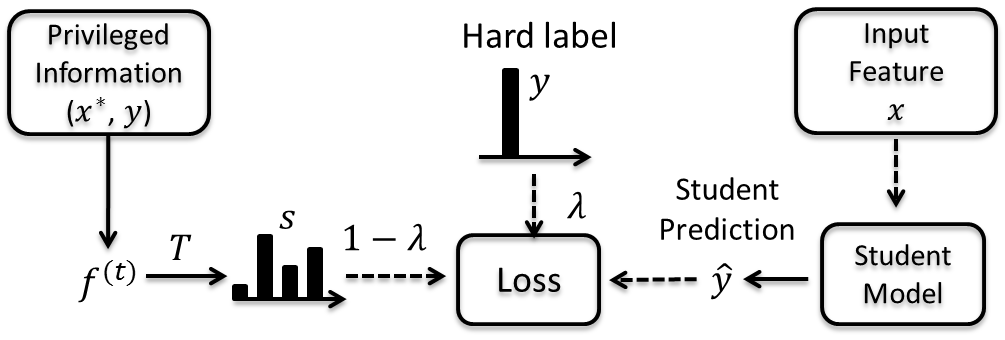
\includegraphics[scale=.35]{figure/GD.png}
	\caption{Illustration of Generalized Distillation training process.}
\end{figure}
%
%
%\textit{Distillation} \cite{hinton2015distilling} and \textit{Learning Using Privileged Information} (LUPI) \cite{vapnik2015learning} are two paradigms that enable machines to learn from other machines. Both methods address the problem of how to build a student model that can learn from the advanced teacher models. Recently, Lopez {et al.} \cite{lopez2015unifying} proposed a framework called \textit{generalized distillation} that unifies both methods and show that it can be applied in many scenarios.
{Generalized Distillation} can be considered as the hybrid of two famous learning paradigms \textit{Distillation}\cite{hinton2015distilling} and \textit{Learning Using Privileged Information}(LUPI)\cite{vapnik2015learning}.
In GD, the training data can be represented as a collection of triples:
\[\{\left(x_1,x_1^*,y_1\right),\left(x_2,x_2^*,y_2\right) \dots \left(x_n,x_n^*,y_n\right)\}\]
$x^*$ is the privileged information for data $x$, which is only available in the training process and $y$ is the corresponding label. 
The process of generalized distillation is as follows: in step 1, a teacher model ${f}^{(t)}$ is trained using the input-output pairs $\{x^*_i,y_i\}_{i=1}^n$. In step 2, ${f}^{(t)}$ is used to generate the soft label $s_i$ for each training example $x_i$ using the softmax function $\sigma$:
\begin{equation}\label{eq:softmax_T}
s_i=\sigma(f^{(t)}(x_i)/T)
\end{equation}
where $T$ is a hyperparameter called \textit{temperature} to control the smoothness of the soft label. In step 3, the student ${f}^{(s)}$ is learned from the pairs $\{\left(x_i,y_i\right),\left(x_i,s_i\right)\}_{i=1}^n$ using:
\begin{equation}\label{eq:distill}
\begin{aligned}
f^{(s)}=&\underset{f^{(s)} \in \mathcal{F}^{(s)}}{\arg \min}\frac{1}{n}\sum_{i=1}^{n}\bigg[\lambda\ell\left(y_i,f^{(s)}(x_i)\right)+(1-\lambda)\ell\left(s_i,f^{(s)}(x_i)\right)\bigg]\\
\end{aligned}
\end{equation}
Here, $\ell(\cdot,\cdot)$ is the loss function and $\lambda$ is the \textit{imitation parameter} to balance the importance between the hard label $y_i$ and the soft label $s_i$. When testing, the student model can predict with the data $x$ alone, without the assistance of the privileged information.


%GD can be used in many scenarios such as multi-task learning, semi-supervised learning, and reinforcement learning. 
In domain adaptation, when we consider the source model as the teacher and the predictions of the target data give by the source models as the privileged information,
GD can be naturally applied to SDA. This leads to \textit{Generalized Distillation Semi-supervised Domain Adaptation} (\textbf{GDSDA}). Moreover, in GDSDA, we also consider the multi-source scenario and extend the GD paradigm to fit this scenario. To be consistent with other work in domain adaptation, we use source model and target model to denote the teacher model and the student model in the rest of our paper in GDSDA.

An important issue of applying GD to SDA is that, in Eq. \eqref{eq:distill}, each target example is assigned with a hard label $y$ (true label) and a soft label $s$ (class probabilities from the teacher). However, in SDA, we are not able to obtain the hard labels of the unlabeled data. Here we use the ``fake label" strategy to label the target data: for the labeled examples, we use \textit{one-hot} strategy to encode their labels while using 0s as the labels of the unlabeled examples. Thus, each example in the target domain is assigned with a label. It is arguable that the ``fake label" strategy would introduce extra noise and degrade the performance. However, we will show in our experiment that this noise can be limited by setting a proper value to the imitation parameter and thus, GDSDA can still leverage the source knowledge effectively (See the single source experiment).
\begin{figure}
	\centering
	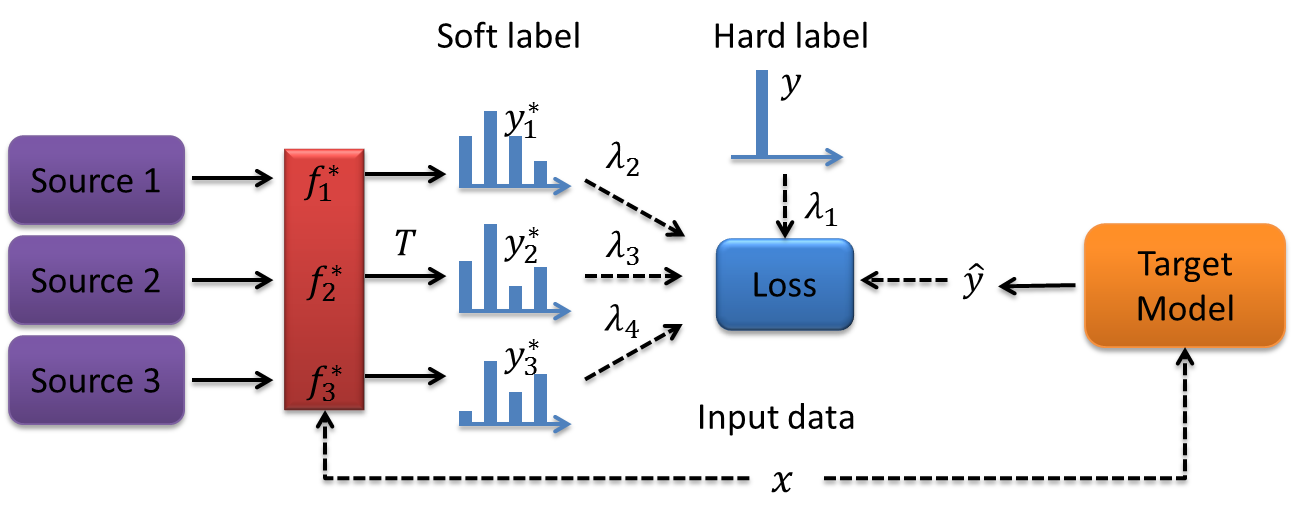
\includegraphics[scale=.4]{figure/multi-GDDA.png}
	\caption{Illustration of GDSDA training process and the ``fake label" strategy.}
	\label{fig:GDSDA}
\end{figure}
 
The process of GDSDA is shown in Figure \ref{fig:GDSDA}. Suppose we have $M-1$ source domains denoted as $D_s^{(j)}=\{X^{(j)},Y^{(j)}\}_{j=1}^{M-1}$ and the target domain $D_t=\{X,Y\}$ encoded with the ``fake label" strategy. The process of GDSDA is as follows:
\begin{enumerate}
    \item Train the source models $f^*_j$ for each of the $M-1$ domains with $\{X^{(j)},Y^{(j)}\}$.
    \item For each of the training example $x_i$ in the target domain, computer the corresponding soft label $y^*_{ij}$ with each of the source model $f^*_j$ and the temperature $T>0$.
    \item Learn the target model $f_t$ with the $(M+1)$-tuples $\{x_i,y_i,y^*_{i1},\dots,y^*_{i(M-1)}\}_{i=1}^L$ and the imitation parameters $\{\lambda_i\}^M_{i=1}$ using \eqref{eq:GDDA_abs}:
\end{enumerate} 
\begin{equation}\label{eq:GDDA_abs}
\begin{aligned}
f_t(\lambda)=\underset{f_t \in \mathcal{F}}{\arg \min}&\frac{1}{L}\sum_{i=1}^{L}\bigg[\lambda_1\ell\left(y_i,f_t(x_i)\right)+\sum_{j=1}^{M-1}\lambda_{j+1}\ell\left(y^*_{ij},f_t(x_i)\right)\bigg]\qquad\\
% &\text{s.t.} \qquad \sum_i\lambda_i=1
\end{aligned}
\end{equation}
Compared to other work of SDA which requires to use each example of the source domain, by either re-weighting \cite{Donahue_2013_CVPR,duan2012visual} or feature augmentation \cite{daume2010frustratingly}, GDSDA only requires the trained model from the source domain to generate the soft labels. 
%Considering the fact that it is more convenient to access the source model than each of the examples of the source domain, GDSDA can be more useful than those previous methods. For example, if we want to use ImageNet \cite{imagenet_cvpr09} as the source domain, it is almost impossible to access each of the millions of the examples while there are many well trained models publicly available online that can be used for GDSDA. 
Meanwhile, GDSDA is able to handle the multi-class scenario while some previous work, such as SHFA\cite{duan2012learning} can only solve the binary classification problem in SDA. Moreover, GDSDA is able to transfer the knowledge from any type of source model that is able to output the soft label (class probabilities) without accessing the source data.

\subsection{Why does GDSDA work}
In this part, we demonstrate the scenario where GDSDA would work. Before we provide our analysis, we first introduce the two basic assumptions of GDSDA: the \textit{assumption of distillation} and \textit{the assumption of the source model}.

\textbf{Assumption of distillation:} \textit{The capacity (VC dimension) of the target model $f_t$ is smaller than the capacity of source model $f^*$.} This assumption is inherited from GD.
\textbf{Assumption of the source model:} \textit{The source model $f^*$ should work better than a target model $f'_t$ trained only with the hard labels.} 
This assumption is based on a simple fact that it is more effective to learn from a superior model. This assumption is very common especially in SDA where the labeled examples are often too few to build a good target model.
For example, when we only have a single labeled example for each class in the target training set, it is reasonable to assume that the source model trained from another domain could outperform a model trained only with the target training data on the target task. %Based on this two assumptions, we will show that GDSDA can effectively leverage the source model and transfer the knowledge between different domains under the SDA setting.

Suppose the complex source model $f^*$ can generalize well on target domain. The simple target model $f_t$ that has the similar training error to the source model $f^*$ would typically do better than the source model $f^*$ itself as well as the target model trained only with hard labels on the target domain (according to the assumption of the source model). This indicates the knowledge can be transferred smoothly between models. Specifically, as it is suggested in \cite{hinton2015distilling}, the transfer process can be achieved by letting the target model mimick the outputs of the source model (soft labels) on the training set without considering the true labels of the training examples. In another word, the source knowledge can be effectively transferred with the unlabeled data.

As the source models are trained from the source domains, it is necessary to weigh the source knowledge due to the domain shift\cite{karl2001long} when we apply it to the target domain. In Eq. \eqref{eq:GDDA_abs}, we use the imitation parameter to control the relative importance between the soft labels and the hard labels, which in turn reflects the amount of the knowledge transferred from each of the source models. Specifically, the larger the imitation parameter, the more important the soft labels are and more knowledge can be transferred from the source domains. 
For example, in Figure \ref{fig:GDSDA}, when we set $\lambda_2=0$, we actually ignore the knowledge from source domain 1.
As a result, with the proper imitation parameter, GDSDA can effectively transfer the knowledge from each of the source models under the setting of SDA (for more details, please see the experiment section).

How to choose the imitation parameter is essential for GDSDA.
Many previous studies have addressed the importance of knowledge transfer control in domain adaptation\cite{duan2012learning,duan2012visual}. Without carefully controlling the amount of knowledge transferred from the source domain, the target model can easily get degraded performance or even suffer from negative transfer\cite{pan2010survey}. However, in the previous studies, the imitation parameter can only be determined by either brute force search\cite{lopez2015unifying} or background knowledge\cite{Tzeng_2015_ICCV} which scale poorly with the number of available source models and imitation parameters.
In this paper, we propose our method, called GDSDA-SVM that can estimate the transfer parameter efficiently.

%In the following, we show that we should choose the imitation parameter that minimizes the empirical risk on the training data for distillation.

%Let $f(x,\lambda)$ be a function with a finite VC dimension $h$ that minimizes the number of errors on the training data $\{x_i,y_i\}_{i=1}^L$. Let $v(\lambda)$ be the training error. Then according to the VC theory \cite{vapnik1999overview}, for an arbitrary loss function $\mathcal{L}(\cdot)$ we have the following bound:
%\begin{equation}\label{eq:lambda_constraint}
%P\left(\mathcal{L}\left(y,f(x,\lambda)\right)\geq 0\right) < v(\lambda)+O\left(\sqrt{\frac{h}{L}}\right)
%\end{equation}
%In other word, the optimal imitation parameter should be the one that can minimize the training error.  

%In the previous work, the imitation parameter can only be determined by either brute force search \cite{lopez2015unifying} or background knowledge \cite{Tzeng_2015_ICCV} which greatly reduces its effectiveness. In domain adaptation, it is common that there could be multiple source models to be exploited. It is ideal to find a method that can determine the imitation parameter automatically.


\section{GDSDA-SVM}\label{sec:svm}
%As we mentioned above, to achieve the best performance of the target model, the imitation parameter should be set to minimize the training error. 
In this section, we propose our method GDSDA-SVM that uses SVM as the base classifier and can effectively estimate the imitation parameter.
\subsection{Distillation with multiple sources}
As we have mentioned previously, imitation parameter is a hyperparameter in GDSDA. A common method to estimate the hyperparameter is to use the cross-validation.
Here we show that it is possible to obtain a closed form cross-validation error\cite{cawley2006leave} in GDSDA-SVM.
As a result,  GDSDA-SVM can estimate the imitation parameter effectively with the gradient descent method.

In our GDSDA-SVM, instead of using hinge loss, we use Mean Squared Error (MSE) as our loss function to train the GDSDA-SVM for the following two reasons: (1) Many recently studies \cite{ba2014deep,luo2016face,romero2014fitnets,urban2016deep} show that MSE is an efficient measurement to let the target model distill the knowledge from the source model. (2) MSE can provide a closed form cross-validation error estimation, so we can estimate the imitation parameter more effectively. 

Suppose we have $L$ examples $\{\textbf{x}_j,\textbf{y}_j\}_{j=1}^L$ from $N$ classes in the target domain where $X\in R^{L\times d}, Y\in R^{L\times N}$. Meanwhile, there are $M-1$ the source (teacher) models providing the soft labels $Y^*=\{\textbf{y}^*_{ij}|j=1,...,L;i=1,...,M-1\}$ for each of the $L$ examples.
For simplicity, we combine the hard label $Y$ and soft label $Y^*$ and use a new label matrix $S$ to denote them, where:
\[S=[Y;Y^*]=[Y_1;...;Y_M]; S \in R^{L\times M \times N}\]
To solve this $N$-class classification problem, we build $N$ binary SVMs.
To obtain the $n$th binary SVM, we have to solve the following optimization problem: 
\begin{equation}\label{eq:multi-distill}
\begin{aligned}
\min \qquad & \frac{1}{2}{|| \textbf{w}_n ||^2} + C\sum_{i,j} \lambda_i{e_{ijn}^2} \quad
s.t. & e_{ijn} = s_{ijn} - \textbf{w}_n\textbf{x}_j;\sum_i\lambda_i=1;\\
%& \sum_i\lambda_i=1; \lambda_i \in [0,1]; i\in M;  j\in L\\
\end{aligned}  
\end{equation}
%To solve this optimization problem, we use KKT theorem \cite{cristianini2000introduction} and add the dual sets of variables to the Lagrangian of the optimization problem:
%\begin{equation}
%\begin{aligned}
%\mathcal{L}=&\frac{1}{2}{|| \textbf{w}_n ||^2} + C\sum_{i,j} \lambda_i{e_{ijn}^2}+\sum_{i,j}\alpha^{(n)}_{ij}\left(s_{ij} - \textbf{w}_n\textbf{x}_j-e_{ij}\right)+\beta^{(n)}\left(\sum_i\lambda_i-1\right)
%\end{aligned}
%\end{equation}
To find the saddle point, 
\begin{equation}
\begin{aligned}
\frac{{\partial L}}{{\partial \textbf{w}_n}}& =0 \rightarrow \textbf{w}_n = \sum_{j}\alpha^{(n)}_{ij} {\textbf{x}_j}; &
\frac{{\partial L}}{{\partial {e_{ijn}}}} & =0 \rightarrow \alpha^{(n)}_{ij} = 2C\lambda_i {e_{ijn}}\\
\end{aligned}
\end{equation}
For each example $\textbf{x}_j$ and its constraint of label $s_{ijn}$, we have $e_{ijn}  + \textbf{w}_n\textbf{x}_j= s_{ijn}$. Replacing $\textbf{w}_n$ and $e_{ijn}$,  we have:  
\begin{equation}
\begin{aligned}
%x_j\sum_{k}\alpha^{(n)}_{ik}x_k+\frac{\alpha^{(n)}_{ij}}{2C\lambda_i}&=s_{ijn}\\
\lambda_i\textbf{x}_j\sum_{k}\alpha^{(n)}_{ik}\textbf{x}_k+\frac{\alpha^{(n)}_{ij}}{2C}&=\lambda_is_{ijn}
%x_j\sum_{k}\alpha^{(n)}_{ik}x_k+\sum_j\frac{\alpha^{(n)}_{ij}}{2C}&=\sum_j\lambda_js_{ijn}
\end{aligned}
\end{equation}
Summing over each constraint of example $x_j$ and let 
$\eta_{jn}=\sum_i\alpha^{(n)}_{ij}$, we have:
%\begin{equation}
%\underbrace{\sum_i\lambda_i}_{=1} \textbf{x}_j\sum_{k}\alpha^{(n)}_{ik}\textbf{x}_k+\sum_i\frac{\alpha^{(n)}_{ij}}{2C}=\sum_i\lambda_is_{ijn}
%\end{equation}
%%Here we use $K$ to denote the kernel matrix $K=\{x_ix_j|i,j\in 1\dots L\}$.
%Let %$M=[K+\frac{\mathbf{I}}{2C}]$ and 
%$\eta_{jn}=\sum_i\alpha^{(n)}_{ij}$, we have:
\begin{equation}
\begin{aligned}
\sum_j\eta_{jn}\textbf{x}_jx_i+\frac{\eta_{in}}{2C}&=\sum_i\lambda_is_{ijn}\\
%M\eta_n&=S_n\begin{bmatrix}
%\lambda_1\\\vdots\\\lambda_m
%\end{bmatrix}
\end{aligned}
\end{equation}

This indicates that solving the optimization problem \eqref{eq:multi-distill} is equivalent to solving a standard SVM whose the target is the weighted sum of each label $\sum_i\lambda_is_{ijn}$.

Here we use $\Omega$ to denote the matrix $\Omega=[K+\frac{\mathbf{I}}{2C}]$ where $K$ is the linear kernel matrix $K=\{\textbf{x}_i\textbf{x}_j|i,j\in 1\dots L\}$. To simplify our notation, let ${\eta}'_{n}=M^{-1}S_n$ where $S_n$ is the matrix $S_n=\{s_{ijn}|i\in M;j\in L\}$ and $\Omega^{-1}$ is the inverse of matrix $\Omega$. 

Let $\eta_{jn}=\sum_i\lambda_i{\eta}'_{ijn}$.
According to  \cite{cawley2006leave}, the Leave-one-out estimation of the example $\textbf{x}_j$ for the $n$th binary SVM can be written as:
%\[\sum_i\lambda_is_{ijn}-\hat{y}_{jn} =\frac{{\eta}_{jn}}{\Omega_{jj}^{-1}} =\frac{\sum_i\lambda_i{\eta}'_{ijn}}{\Omega_{jj}^{-1}}\]
\begin{equation}\label{eq:yhat}
\hat{y}_{jn} = \sum_i\lambda_i\left(s_{ijn}-\frac{{\eta}'_{ijn}}{\Omega_{jj}^{-1}}\right)
\end{equation}
where $\Omega^{-1}_{jj}$ is the $j$th diagonal element of $\Omega^{-1}$.
% Now for any given $\lambda$, we have found an efficient way to estimate the LOO of each binary target model for example $\textbf{x}_j$. 
%In the following part, we will introduce how to find the optimal $\lambda_i$ for each of the source models. 
\subsection{Cross-entropy loss for imitation parameter estimation}
From the previous part, we have already found a effective way to calculate the leave-one-out estimation of the target model. The optimal imitation parameters can be found by minimizing the leave-one-out cross-validation error on the target data:
\begin{equation}\label{eq:loo_loss}
\begin{aligned}
\min \quad& L_c\left(\lambda\right)=\frac{1}{2}\sum_i^M||\lambda_i||^2+\frac{1}{L}\sum_{j,n}\ell\left(y_{in},\hat{y}_{jn}\left(\lambda\right)\right) &
s.t. \quad& \sum\lambda_i=1
\end{aligned}
\end{equation}
Here we use the $\ell$-2 regularization term to control the complexity of $\lambda$ so that the target model can achieve better generalization performance even with a small training set. For the loss function $\ell(\cdot,\cdot)$, we use the cross-entropy loss function.
\begin{equation}\label{eq:ce}
\begin{aligned}
\ell\left(y_{in},\hat{y}_{jn}\left(\lambda\right)\right)=&y_{in}\log(P_{jn}) & for \quad&
P_{jn} = \frac{e^{\hat{y}_{jn}}}{\sum_{h} e^{\hat{y}_{jh}}}
\end{aligned}
\end{equation}
Typically, cross-entropy pays less attention to a single incorrect prediction which reduces the affect of the outliers of the training data. Moreover, cross-entropy has its own advantage with our "fake label" strategy. As we have mentioned previously, we use gray code to encode the unlabeled examples. When we use cross-entropy loss, it can automatically ignore penalties of the unlabeled examples and reduce the affect of the noise introduced by our "fake label" strategy. 
%Let:
%\begin{equation}\label{eq:mu}
%\begin{aligned}
%\mu_{ijn}=s_{ijn}-\frac{{\eta}'_{ijn}}{\Omega_{jj}^{-1}} \qquad
%\end{aligned}
%\end{equation}
As a result, the derivative of Eq. \eqref{eq:ce} can be calculated as:
\begin{equation}\label{eq:p}
\begin{aligned}
\frac{\partial \ell(\lambda)}{\partial \lambda_i}&=\sum_n\bigg(s_{ijn}-\frac{{\eta}'_{ijn}}{\Omega_{jj}^{-1}}\bigg)\left(P_{jn}-{y}_{jn}\right)
\end{aligned}
\end{equation}
\begin{algorithm}[t]
	\caption{GDSDA-SVM}\label{alg:svm}
	\begin{algorithmic}
		\REQUIRE Input examples $X=\{\textbf{x}_1,...,\textbf{x}_L\}$, number of classes $N$, number of sources $M$, 3-D label matrix, $S=[Y_1,Y_2,...,Y_{M}]$ with size $L\times M \times N$, temperature $T$ %optimization iteration $iter$
		\ENSURE Target model $f_t = Wx$
		\STATE Compute $\Omega=[K+\frac{\mathbf{I}}{2C}]$
		\STATE Compute imitation parameter $\lambda$ with Algorithm \ref{alg:lambda}
		\STATE Generate the new label $Y_{new}=\sum_i\lambda_iY_i$
		\STATE Compute $\eta = \Omega^{-1}Y_{new}$
		\STATE Compute $w_n = \sum_j \eta_{jn}x_j$
	\end{algorithmic}	
\end{algorithm}
\begin{algorithm}[t]
	\caption{$\lambda$ Optimization}\label{alg:lambda}
\begin{algorithmic}
	\REQUIRE Input examples $X$, number of classes $N$, size of sources $M$, 3D label matrix $S$,  optimization iteration $iter$, Kernel matrix $\Omega$
    \ENSURE Imitation parameter $\lambda$
    \STATE Initialize $\lambda = \frac{1}{M}$, 
    
    \STATE Let $S_n$ be the label matrix of $S$ for class $n$
    \FOR{Each label $S_n$} 
    \STATE Compute $\eta'_n=\Omega^{-1}S_n$ 
    \ENDFOR
%    \STATE Compute $\mu_{ijn}=s_{ijn}-\frac{{\eta}'_{ijn}}{\Omega_{jj}^{-1}}$
    \FOR {$it \in \{1,...,iter\}$ }
	    \STATE Compute $\hat{y}_{jn}$ and $P_{jn}$ with \eqref{eq:yhat}  and \eqref{eq:ce}
%	    \STATE $\Delta_{\lambda} \leftarrow 0$
	    \FOR {each $\textbf{x}_j$ in $X$}
		    \STATE $\Delta_{\lambda} = \Delta_{\lambda}+\sum_n\bigg(s_{ijn}-\frac{{\eta}'_{ijn}}{\Omega_{jj}^{-1}}\bigg)\left(P_{jn}-{y}_{jn}\right)$
	    \ENDFOR
	    \STATE $\Delta_{\lambda} =\Delta_{\lambda}/L$, $\lambda = \lambda - \frac{1}{it}(\Delta_{\lambda}+\lambda)$
	    , $\lambda = \lambda / \sum\lambda_i$
%	    \STATE 
    \ENDFOR
\end{algorithmic}	
\end{algorithm}

To summarize, we describe GDSDA-SVM in Algorithm \ref{alg:svm}. As the optimization problem \eqref{eq:loo_loss} is strongly convex, we can prove that Algorithm \ref{alg:lambda} can converge to the optimal $\lambda$ with the rate of $O(\log(t)/t)$ where $t$ is the optimization iteration (We are not able to show our proof here due to the space limit). 






\section{Experiments}\label{sec:exp}
In this section, we show the empirical performance of our algorithm GDSDA-SVM on the Office benchmark dataset. Specifically, we provide two scenarios: single source and multi-source transfer scenario for GDSDA-SVM.

\textbf{Dataset:}
There are 3 subsets in Office datasets, Webcam (795 examples), Amazon (2817 examples) and DSLR (498 examples), sharing 31 classes. We denote them as W, A and D respectively. In our experiments, we use DSLR and Webcam as the source domains and Amazon as the target domain.
We use the features extracted from Alexnet \cite{KrizhevskyNIPS12} FC7 as the input features for both source and target domain. The source models are trained with multi-layer perception (MLP) on the whole source dataset. 

\subsection{Single Source for Office datasets}
In this experiment, we compare our algorithm under the scenario where the source model is trained from a single source dataset. Specifically, we have two groups of experiments, transferring from Webcam to Amazon and from DSLR to Amazon. As we mentioned, there are significantly fewer labeled examples than unlabeled ones in real SDA applications.
Therefore, in each group of experiment, there are only 31 labeled examples (1 per class) and some unlabeled examples (10, 15 and 20 per class) in the target domain to train the target model.
%we set the size of the labeled example to be 1 per class, and the size of the unlabeled example to be 10, 15 and 20 per class respectively.

To demonstrate the effectiveness of GDSDA-SVM, we show the performance of GDSDA using brute force to search the imitation parameter as the baseline. As there are two imitation parameters in this experiment, we use $\lambda_1$ and  $1-\lambda_1$ to denote the imitation parameter for hard and soft label respectively. Specifically, we search the imitation parameter $\lambda_1$ in the range $[0,0.1,...,1]$ with different temperature $T$. Meanwhile, we show the performance of the source model (denoted as ``Source") and the performance of a target model (denoted as ``No transfer" using LIBLINEAR\cite{fan2008liblinear}) trained with only labeled examples of the target domain\footnote{We failed to achieve a better performance using semi-supervised learning method \cite{delalleau2005efficient} on the target data as the no transfer baseline (may due to the size of the initial labeled examples).} on the target task. We perform each experiment 10 times and report the average result. For GDSDA-SVM, as we are not able to tune the temperature $T$, we empirically set $T=20$  and $\beta=1$ for all experiments in this part. The experimental results are shown in Figure \ref{fig:single1}. 
%$\lambda$ on the X-axis of the figures denotes the imitation parameter for the hard label and the corresponding imitation parameter for the soft label is set to $1-\lambda$.

From the results of brutal force search we can see that, the value of imitation parameter can greatly affect the performance of the target model.
Also without using any label information of the target data for distillation, i.e. $\lambda_1 = 0$, as we expected, GDSDA can still slightly outperform the source model. This means GDSDA can effectively transfer the knowledge between different domains with the unlabeled data. As we increase the value of imitation parameter, i.e. introducing the hard labels from the target domain, the performance of GDSDA can be further improved. As we mentioned before, even though our ``fake label" strategy would introduce extra noise, the noise can be limited by setting a proper value to imitation parameter and the target model can still get improved performance compared to the baselines.

Moreover, we can see that GDSDA-SVM can achieve competitive results compared to baselines using brutal force search in D$\rightarrow$A experiments. In W$\rightarrow$A experiments, it achieves the best performances on all 3 different unlabeled sizes. This indicates that we can efficiently (about 6 times faster than brutal force search) obtain a good target model with GDSDA-SVM.
%\newpage
%\subsubsection{From DSLR to Amazon}
\begin{figure}[t]
\centering
\begin{tabular}{cccc}
\subfloat[D $\rightarrow$ A, 10 unlabeled ]{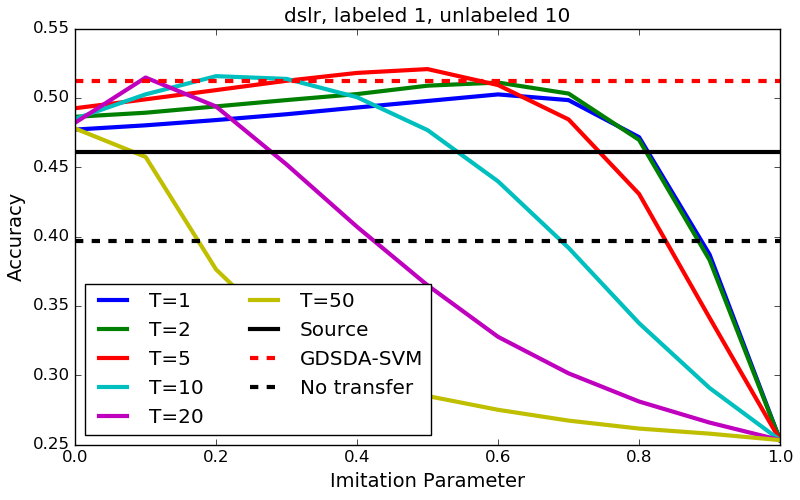
\includegraphics[width=0.3\textwidth]{figure/dslrtoamazonlabeled1unlabeled10.png}}&
\subfloat[D $\rightarrow$ A, 15 unlabeled ]{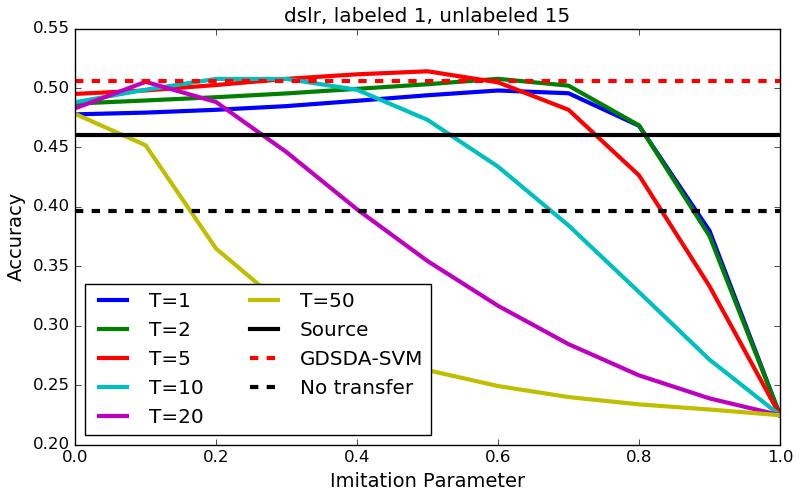
\includegraphics[width=0.3\textwidth]{figure/dslrtoamazonlabeled1unlabeled15.png}}&
\subfloat[D $\rightarrow$ A, 20 unlabeled ]{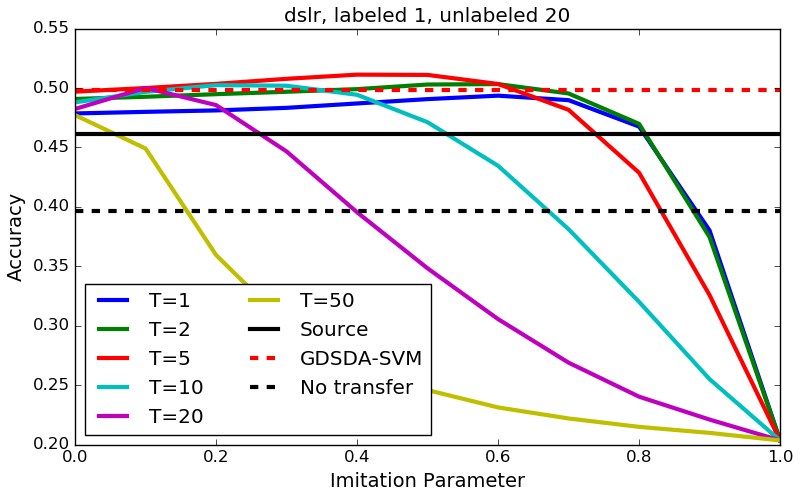
\includegraphics[width=0.3\textwidth]{figure/dslrtoamazonlabeled1unlabeled20.png}}\\
\subfloat[W $\rightarrow$ A, 10 unlabeled ]{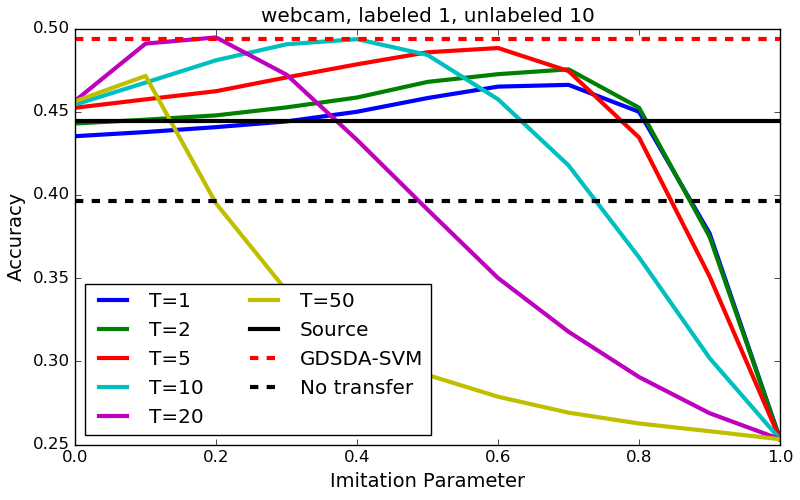
\includegraphics[width=0.3\textwidth]{figure/webcamtoamazonlabeled1unlabeled10.png}}&
\subfloat[W $\rightarrow$ A, 15 unlabeled ]{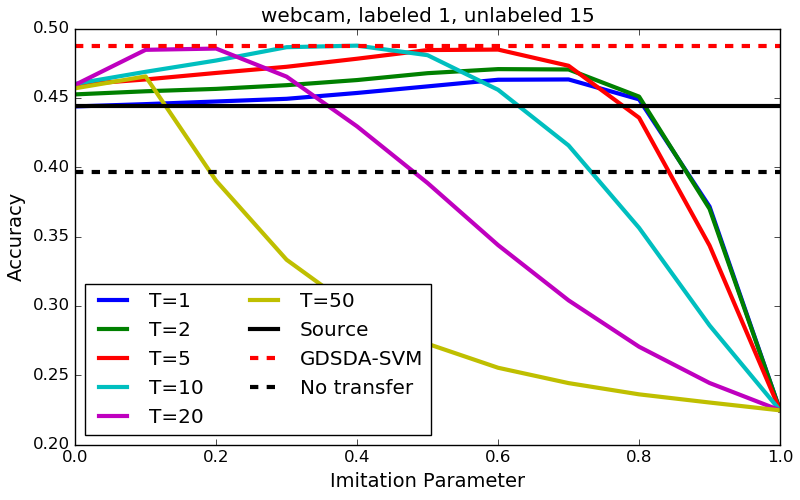
\includegraphics[width=0.3\textwidth]{figure/webcamtoamazonlabeled1unlabeled15.png}}&
\subfloat[W $\rightarrow$ A, 20 unlabeled ]{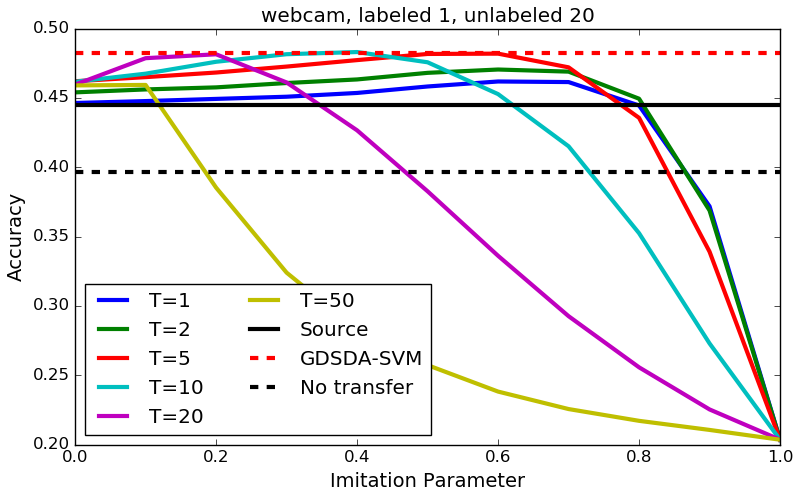
\includegraphics[width=0.3\textwidth]{figure/webcamtoamazonlabeled1unlabeled20.png}}\\
\end{tabular}
\caption{Experiment results on DSLR$\rightarrow$Amazon and Webcam$\rightarrow$Amazon when there are just one labeled examples per class. The results of DSLR$\rightarrow$Amazon and Webcam$\rightarrow$Amazon are shown in figure (a)-(c) and (d)-(e) respectively. GDSDA-SVM is trained with temperature $T=20$. The X-axis denotes the imitation parameter of the hard label (i.e. $\lambda_1$ in Fig \ref{fig:GDSDA}) and the corresponding imitation parameter of the soft label is set to $1-\lambda_1$.
}\label{fig:single1}
\end{figure}
\subsection{Multi-Source for Office datasets}
\begin{figure}
	\centering
	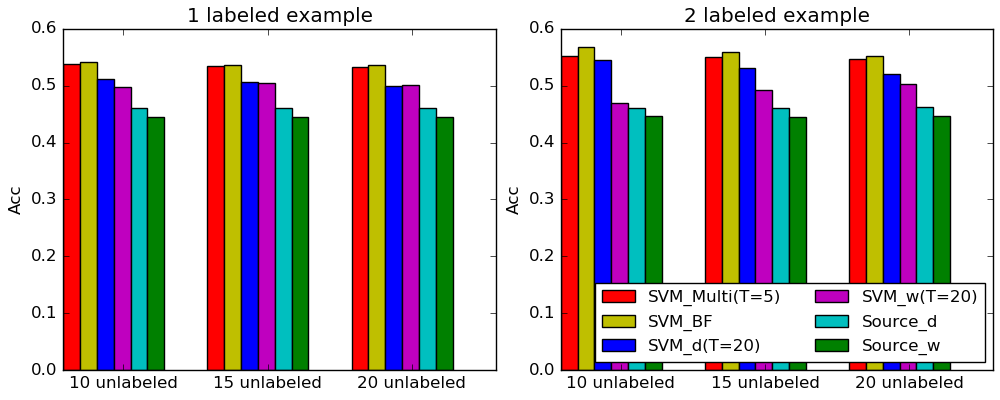
\includegraphics[scale=.34]{figure/cmp.png}
	\caption{D+W$\rightarrow$A, Multi-source results comparison.}\label{fig:multi}
\end{figure}
In this experiment, we show the performance of GDSDA-SVM under the multi-source SDA scenario.
Specifically, we use Amazon as the target domain and the target domain can leverage the knowledge of two source models trained from Webcam and DSLR.
We use the similar settings as our single source experiment and perform 2 groups of experiments using 1 labeled and 2 labeled examples per class respectively. We use temperature $T=5$ and set and $\beta=1$. The results of multi-source GDSDA-SVM are denoted as SVM\_Multi. Here we also include two single source GDSDA-SVMs obtained from the experiments above (SVM\_w and SVM\_d trained using Webcam and DSLR as the source respectively) as the baselines. Moreover, we show the best performance of the brutal force search model (SVM\_BF). For SVM\_BF, we search temperature in range $T=[1,2,5,10,20,50]$ and each imitation parameter in range $[0,0.1,...,1]$. The experiment results are shown in Figure \ref{fig:multi}.

From the results, we can see that, given 2 source models, SVM\_Multi can outperform any single source model trained with GDSDA. This indicates GDSDA-SVM can still exploit the knowledge even in the complex multi-source scenario. Even though SVM\_Multi performs slightly worse than the best result found by brutal force search in some experiments, considering their time consumption (GDSDA-SVM is around 30 times faster than brutal force search), SVM\_Multi still has its advantage in real applications.






\section{Conclusion}\label{sec:con}
In this paper, we propose a framework called {Generalized Distillation Semi-supervised Domain Adaptation} that can effectively leverage the knowledge from the source domain using the unlabeled data of the SDA problem. To make GDSDA more effective in real applications, we proposed a method called GDSDA-SVM and show that GDSDA-SVM can effectively estimate the imitation parameter for GDSDA. Experiment results show that GDSDA-SVM can effectively leverage the knowledge from one or more source models for the real SDA applications.



\bibliographystyle{splncs03}
\bibliography{research}


%\bibauthoryear

\end{document}
